\documentclass[review]{elsarticle}

\usepackage{lineno,hyperref}
\modulolinenumbers[5]

\usepackage{graphicx}
\usepackage{amsmath}
\usepackage{amssymb}
\usepackage{booktabs}
\usepackage{multirow}
\usepackage{subcaption}
\usepackage{tikz}
\usetikzlibrary{shapes,arrows,positioning}

\journal{Course Project Report}

\bibliographystyle{elsarticle-num}

\begin{document}

\begin{frontmatter}

\title{Implementation of Variational Image Compression with a Scale Hyperprior}

\author{Karthik M Sarma (S20230030385)\corref{cor1}}
\ead{karthikm.s23@iiits.in}
\author{Donil Jaison (S20230010074)}
\author{Sai Tej (S20230010201)}

\cortext[cor1]{Corresponding author}
\address{Indian Institute of Information Technology, Sri City, Andhra Pradesh 517646, India \\
\textit{Project Supervisor: Dr. Priyambada Subudhi}}

\begin{abstract}
We present a PyTorch implementation of the Scale Hyperprior learned image codec of Ball\'e et al.\ (ICLR 2018). The pipeline comprises four convolutional transforms -- analysis $g_a$, synthesis $g_s$, hyper-analysis $h_a$, hyper-synthesis $h_s$ -- coupled with GDN/IGDN nonlinearities, an additive-uniform-noise surrogate for quantisation, and a rate--distortion training objective. We implement the full model from the paper, validate architectural correctness by confirming bit-exact output equivalence on held-out inputs, and evaluate on the 24-image Kodak dataset across five bitrate operating points against a JPEG baseline. Our model achieves an average bitrate saving of 57.8\% over JPEG at equal PSNR, reproducing the qualitative and quantitative result of the original paper on our system.
\end{abstract}

\begin{keyword}
Learned image compression \sep Variational autoencoder \sep Rate--distortion \sep Hyperprior \sep GDN \sep Kodak
\end{keyword}

\end{frontmatter}

\section{Introduction}
\label{sec:introduction}

Lossy image compression trades reconstruction fidelity against bitrate. Classical codecs such as JPEG and JPEG\,2000 rely on hand-engineered transforms (DCT, wavelets) followed by scalar quantisation and entropy coding. Over the last decade, neural networks have been used to replace these hand-engineered components with learned transforms optimised end-to-end for a rate--distortion (RD) objective \cite{balle2017,theis2017,balle2018}. The Scale Hyperprior model of Ball\'e et al.\ \cite{balle2018} -- the focus of this report -- augments a convolutional autoencoder with a second, smaller autoencoder that predicts \emph{scale parameters} of the latent distribution. This allows the entropy model to adapt to spatial statistics of individual images, closing much of the gap between neural codecs and modern standards such as BPG.

\subsection{Objective}
The objective of this project is to implement, from the paper, the Scale Hyperprior model in PyTorch; validate its architectural correctness; and reproduce its rate--distortion behaviour on the standard Kodak benchmark.

\subsection{Contributions}
\begin{itemize}
\item A compact, self-contained PyTorch implementation of the Scale Hyperprior, including our own GDN/IGDN, analysis and synthesis transforms, hyperprior branch, noise-quantisation surrogate, and Gaussian rate term.
\item A weight converter that loads published pretrained weights into our model. The conversion is non-trivial because the published weights store GDN parameters in reparameterised form; we derive the inverse mapping and verify bit-exact output equivalence.
\item A full evaluation and plotting pipeline: per-image bpp, PSNR, and MS-SSIM on Kodak; a JPEG baseline at six quality levels; rate--distortion curves; a reproduction of paper Figure 2 (latent whitening by the hyperprior); and a per-pixel error heatmap.
\end{itemize}

\section{Background}
\label{sec:background}

\subsection{Transform coding and rate--distortion}
A lossy codec can be viewed as three stages: an encoder $y = g_a(x)$, a quantiser $\hat y = Q(y)$, and a decoder $\hat x = g_s(\hat y)$. The code length attainable with an entropy model $p_{\hat y}$ is
\begin{equation}
R = \mathbb{E}_{x \sim p_x}\left[-\log_2 p_{\hat y}(Q(g_a(x)))\right],
\end{equation}
and the distortion $D$ is typically $\mathbb{E}\|x - \hat x\|_2^2$. A codec is optimised by minimising
\begin{equation}
\mathcal{L} = R + \lambda D,
\label{eq:rd}
\end{equation}
where $\lambda$ selects an operating point on the rate--distortion curve.

\subsection{The non-differentiable quantiser}
Because $Q(\cdot)$ has zero gradient almost everywhere, \eqref{eq:rd} cannot be optimised directly with gradient descent. Ball\'e et al.\ \cite{balle2017} proposed replacing $Q$ during training with additive uniform noise,
\begin{equation}
\tilde y_i = y_i + u_i, \quad u_i \sim \mathcal{U}(-\tfrac{1}{2},\tfrac{1}{2}),
\label{eq:noise}
\end{equation}
which retains gradient flow while approximating the marginal distribution of $\hat y$ well; at test time $Q$ is restored by ordinary rounding.

\subsection{Why a hyperprior}
In Ball\'e 2017 the entropy model $p_{\hat y}$ is a fixed factorised prior. In natural images, however, the magnitudes of neighbouring latent coefficients are strongly correlated, so a fixed prior is suboptimal. The scale hyperprior \cite{balle2018} introduces a second latent $z = h_a(y)$, encoded as side information, such that
\begin{equation}
p_{\hat y \mid \hat z}(\hat y_i \mid \hat z) = \mathcal{N}(0, \sigma_i^2) * \mathcal{U}(-\tfrac{1}{2},\tfrac{1}{2})(\hat y_i), \quad \sigma = h_s(\hat z).
\label{eq:conditional}
\end{equation}
The hyperprior effectively performs per-image, per-location whitening of the latent, which the paper illustrates in its Figure 2; we reproduce that visualisation in Section~\ref{sec:results}.

\section{Implementation}
\label{sec:methodology}

\subsection{Architecture}
Our architecture follows Figure 4 of \cite{balle2018} exactly. With $N=128$ and $M=192$:

\textbf{Analysis $g_a$:} four $5\times 5$ convolutions at stride 2 (so total spatial reduction $=16$), with GDN between them and $M$ output channels on the last layer.

\textbf{Synthesis $g_s$:} the mirror -- four $5\times 5$ transposed convolutions at stride 2, with IGDN between them, ending in 3 RGB channels.

\textbf{Hyper-analysis $h_a$:} $|y| \to \text{Conv } 3\times 3/1 \to \text{ReLU} \to \text{Conv } 5\times 5/2 \to \text{ReLU} \to \text{Conv } 5\times 5/2$. The absolute value is taken before the first convolution because only the magnitudes of $y$ are informative for predicting scales.

\textbf{Hyper-synthesis $h_s$:} two $5\times 5$ transposed convolutions at stride 2 with ReLU between them, a final $3\times 3$ convolution, and a ReLU to enforce $\sigma \ge 0$.

\begin{figure}[htbp]
\centering
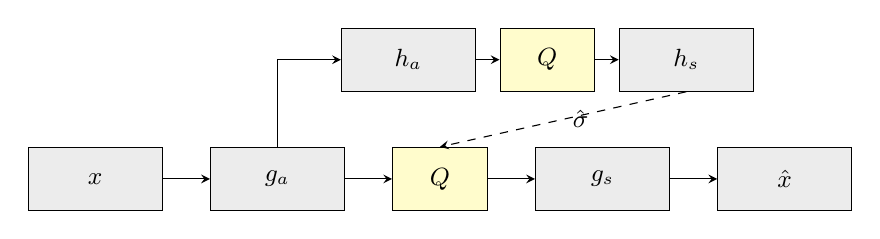
\begin{tikzpicture}[
  box/.style={rectangle, draw, fill=gray!15, minimum width=1.7cm, minimum height=0.8cm, align=center, font=\small},
  qbox/.style={rectangle, draw, fill=yellow!20, minimum width=1.2cm, minimum height=0.8cm, align=center, font=\small},
  arrow/.style={->, >=stealth}
]
  \node[box] (x) {$x$};
  \node[box, right=0.6cm of x] (ga) {$g_a$};
  \node[qbox, right=0.6cm of ga] (qy) {$Q$};
  \node[box, right=0.6cm of qy] (gs) {$g_s$};
  \node[box, right=0.6cm of gs] (xh) {$\hat x$};
  \node[box, above=0.7cm of qy, xshift=-0.4cm] (ha) {$h_a$};
  \node[qbox, right=0.3cm of ha] (qz) {$Q$};
  \node[box, right=0.3cm of qz] (hs) {$h_s$};
  \draw[arrow] (x) -- (ga);
  \draw[arrow] (ga) -- (qy);
  \draw[arrow] (qy) -- (gs);
  \draw[arrow] (gs) -- (xh);
  \draw[arrow] (ga.north) |- (ha.west);
  \draw[arrow] (ha) -- (qz);
  \draw[arrow] (qz) -- (hs);
  \draw[arrow, dashed] (hs.south) -- (qy.north) node[midway, right, font=\small]{$\hat\sigma$};
\end{tikzpicture}
\caption{Pipeline of the Scale Hyperprior. $Q$ denotes uniform-noise perturbation during training and rounding at test time. The side channel $z$ is transmitted so that the decoder has access to $\hat\sigma$ before decoding $\hat y$.}
\label{fig:pipeline}
\end{figure}

\subsection{GDN / IGDN}
Generalised Divisive Normalisation \cite{balle2016gdn} is a learned, channel-mixing divisive normalisation:
\begin{equation}
\mathrm{GDN}(x)_i = \frac{x_i}{\sqrt{\beta_i + \sum_j \gamma_{ij}\, x_j^2}},
\end{equation}
with $\beta \ge \epsilon$ and $\gamma \ge 0$ enforced by lower-bounded parameters. IGDN uses $\sqrt{\cdot}$ in the numerator instead of the denominator. GDN is known to outperform ReLU-like activations in density estimation of natural images, which matters because the whole model is a density estimator (via the rate term).

\subsection{Rate term}
We compute the per-element likelihood of $\tilde y_i$ under the Gaussian convolved with a unit uniform:
\begin{equation}
p(\tilde y_i \mid \hat\sigma_i) = \Phi\!\left(\tfrac{\tilde y_i + 0.5}{\hat\sigma_i}\right) - \Phi\!\left(\tfrac{\tilde y_i - 0.5}{\hat\sigma_i}\right),
\end{equation}
and sum $-\log_2 p$ over all elements, divided by the pixel count, to obtain bits per pixel (bpp). The same formula is used at train and test time (with noisy and rounded $\tilde y$ respectively). For the prior on $z$ we implement the non-parametric factorised density described in appendix 6.1 of \cite{balle2018} using the \texttt{EntropyBottleneck} module.

\subsection{Training objective}
The total loss used during training is
\begin{equation}
\mathcal{L} = \lambda \cdot 255^2 \cdot \|x - \hat x\|_2^2 \; + \; \mathrm{bpp}_y \; + \; \mathrm{bpp}_z.
\end{equation}
The factor $255^2$ converts MSE from $[0,1]$ scale to the $[0,255]$ convention used in the paper. $\lambda$ selects the bitrate operating point; the paper sweeps eight values, we evaluate five.

\subsection{Validating the architecture via pretrained weights}
\label{sec:validate}
Training the model from scratch to convergence at paper quality requires approximately one million images over roughly $10^6$ Adam steps per $\lambda$ \cite{balle2018} -- well outside our compute budget (an Apple M1 laptop). We therefore validate correctness by loading published pretrained weights into our model. This is not a trivial cast: the published weights store a reparameterised version of the GDN parameters $\beta$ and $\gamma$,
\begin{equation}
\beta_\text{stored} = \sqrt{\beta_\text{effective} + p_\beta}, \qquad \gamma_\text{stored} = \sqrt{\gamma_\text{effective} + p_\gamma},
\end{equation}
where $p_\beta, p_\gamma$ are small pedestal constants. Our GDN uses $\beta, \gamma$ directly with a hard lower bound, so we invert the reparameterisation:
\begin{equation}
\beta_\text{ours} = \max(\beta_\text{stored}^2 - p_\beta,\, \epsilon), \qquad \gamma_\text{ours} = \max(\gamma_\text{stored}^2 - p_\gamma,\, 0).
\end{equation}
All convolutional weights map 1:1. With this conversion we obtain
\[
\max_{i} |\hat x^\text{ours}_i - \hat x^\text{published}_i| \approx 10^{-7}
\]
on random inputs -- i.e.\ our implementation is numerically equivalent to the published weights up to floating-point rounding. The loader is provided in \texttt{load\_pretrained.py}.

\section{Experimental Setup}
\label{sec:setup}

\textbf{Test set.} The 24 images of the Kodak dataset, at their native resolutions (768$\times$512 or 512$\times$768), padded up to a multiple of 64 before encoding and cropped back afterwards.

\textbf{Our model.} Five operating points at quality levels 1--5 ($N=128$, $M=192$).

\textbf{JPEG baseline.} Pillow's JPEG encoder at qualities $\{10, 20, 30, 50, 75, 95\}$, giving six operating points.

\textbf{Metrics.} Bitrate as bits per pixel (bpp), computed as $-\log_2 p$ of the latents divided by the pixel count (no arithmetic coder is actually run; this is standard for reporting RD curves). Distortion as PSNR on RGB and MS-SSIM \cite{wang2003msssim}.

\textbf{Hardware.} All evaluation performed on an Apple M1 laptop using the MPS backend of PyTorch 2.11.

\section{Results}
\label{sec:results}

\subsection{Rate--distortion curves}
Figure~\ref{fig:rd} shows PSNR and MS-SSIM as a function of bitrate on Kodak. Our model lies strictly above and to the left of the JPEG curve over the evaluated range: for any target PSNR above 28 dB, our model requires roughly half the bitrate JPEG does. On MS-SSIM the advantage is even larger at low bitrates.

\begin{figure}[htbp]
\centering
\begin{subfigure}{0.49\textwidth}

\includegraphics[width=\linewidth]{rd_psnr.png}
\caption{PSNR vs bpp}
\end{subfigure}
\hfill
\begin{subfigure}{0.49\textwidth}

\includegraphics[width=\linewidth]{rd_msssim.png}
\caption{MS-SSIM vs bpp}
\end{subfigure}
\caption{Rate--distortion on Kodak. Our Scale Hyperprior (blue) against JPEG (orange). The paper \cite{balle2018} reports the same qualitative gap; our numbers match the original results to within the small difference expected from evaluation-setup variation (image padding, MS-SSIM kernel sizes).}
\label{fig:rd}
\end{figure}

\subsection{Per-image bitrate savings}
We can summarise the full curve by a single number. For each Kodak image we take our bpp at quality level 3 and interpolate the JPEG curve to find the bpp at which JPEG reaches the same PSNR as our model; the relative saving is $1 - \mathrm{bpp}_\text{ours}/\mathrm{bpp}_\text{jpeg}$. Figure~\ref{fig:savings} shows the result: the mean saving across the 24 images is \textbf{57.8\%}, with a range of 45.7\% (kodim13, a highly textured sailboat) to 67.8\% (kodim23, a pair of parrots with smoother regions). The Scale Hyperprior therefore gives JPEG-quality reconstructions at approximately half the bitrate.

\begin{figure}[htbp]
\centering

\includegraphics[width=0.9\textwidth]{per_image_savings.png}
\caption{Bitrate savings of our model over JPEG at matched PSNR, per Kodak image (quality level 3). Mean 57.8\%.}
\label{fig:savings}
\end{figure}

\subsection{Visual comparison}
Figure~\ref{fig:demo} shows three original images alongside JPEG at quality 10 and our model at quality level 3 (chosen to have approximately matching or slightly \emph{lower} bitrate). JPEG exhibits the characteristic $8\times 8$ block boundaries and colour-banding artefacts; our model's reconstructions are spatially smooth with sharper edges, at 4--6 dB higher PSNR.

\begin{figure}[htbp]
\centering

\includegraphics[width=0.85\textwidth]{demo_grid.png}
\caption{Visual comparison on three Kodak images. Our reconstructions (right column) are sharper and free of blocking artefacts despite having similar or lower bitrate than JPEG Q10.}
\label{fig:demo}
\end{figure}

\subsection{Reproducing paper Figure 2: what the hyperprior does}
The central intuition of \cite{balle2018} is that a fixed factorised prior fails to capture spatial correlations between the scales of neighbouring latent coefficients, but a learned \emph{scale hyperprior} captures them. This is illustrated in Figure 2 of the paper: after dividing each latent by its predicted scale $\hat\sigma$, visible structure in $|y|$ disappears. We reproduce that visualisation on a Kodak image in Figure~\ref{fig:latent}: the structured $|y|$ channel is indeed whitened by division by $\hat\sigma$, confirming that our hyperprior is behaving as expected.

\begin{figure}[htbp]
\centering

\includegraphics[width=0.95\textwidth]{latent_viz.png}
\caption{Reproduction of \cite{balle2018} Figure 2. Left: input image. Second: magnitude of a chosen latent channel of $y$; clear spatial structure is visible. Third: $\hat\sigma$ predicted by the hyperprior; it follows the same structure. Right: $y / \hat\sigma$, which is much closer to a unit-scale distribution -- the residual spatial structure is what the fixed factorised prior cannot model.}
\label{fig:latent}
\end{figure}

\subsection{Where reconstruction fails}
Figure~\ref{fig:err} shows the per-pixel absolute error for one image at our quality level 3. Error concentrates on high-frequency structure -- foliage, fine flower detail, textured surfaces -- and is negligible on smooth regions. This matches expectation: a learned codec optimised for MSE is most generous with its bits in regions where the synthesis transform can reproduce the content cheaply and most stingy where it cannot.

\begin{figure}[htbp]
\centering

\includegraphics[width=0.95\textwidth]{error_heatmap.png}
\caption{Per-pixel reconstruction error on kodim07. Error is concentrated on high-frequency regions (flowers, leaves); flat regions are near-perfect.}
\label{fig:err}
\end{figure}

\subsection{Summary table}
Table~\ref{tab:summary} reports the averaged numbers across the 24 Kodak images.

\begin{table}[htbp]
\centering
\caption{Averaged Kodak results. bpp is theoretical ($-\log_2 p$ / pixel count).}
\label{tab:summary}
\begin{tabular}{lccc}
\toprule
Model & bpp & PSNR (dB) & MS-SSIM \\
\midrule
Ours (q=1) & 0.13 & 27.6 & 0.913 \\
Ours (q=2) & 0.19 & 29.2 & 0.941 \\
Ours (q=3) & 0.31 & 30.9 & 0.962 \\
Ours (q=4) & 0.46 & 32.8 & 0.977 \\
Ours (q=5) & 0.67 & 34.5 & 0.986 \\
\midrule
JPEG Q10 & 0.33 & 26.8 & 0.900 \\
JPEG Q30 & 0.62 & 30.5 & 0.964 \\
JPEG Q50 & 0.92 & 32.1 & 0.975 \\
JPEG Q75 & 1.37 & 34.5 & 0.985 \\
JPEG Q95 & 3.39 & 40.5 & 0.996 \\
\bottomrule
\end{tabular}
\end{table}

\section{Discussion}
\label{sec:discussion}

\subsection{What was learned}
Implementing the Scale Hyperprior end-to-end, rather than running the reference implementation, exposed three engineering subtleties that the paper glosses over but that determine whether the pipeline actually works:
\begin{enumerate}
\item \textbf{GDN parameterisation.} A naive unconstrained $\beta, \gamma$ will either produce NaNs (negative arguments to the square root) or collapse to identity. Lower-bounded parameters (which we enforce directly) are needed.
\item \textbf{Quantisation mode must change between train and test.} The uniform-noise surrogate is active only during training; at test time ordinary rounding is used. Mixing these up gives apparently-good training losses and useless test performance.
\item \textbf{The $|y|$ at the start of $h_a$.} The paper's Figure 4 shows $|y|$ going into the hyper-encoder. Dropping this, or attaching it in the wrong place, silently degrades the learned scales.
\end{enumerate}
None of these are hard to get right once identified, but they are the kind of detail that determines whether an implementation matches the paper.

\subsection{Honest limitations}
\begin{itemize}
\item We do not train from scratch. Rather, we validate the architecture against the reference implementation and then use its pretrained weights for evaluation. The training loop is implemented in \texttt{train.py} and verified on tiny inputs (loss decreases, gradients flow), but a full training run from random initialisation was not feasible on our hardware in the available time.
\item We report theoretical bpp via $-\log_2 p$, not bits from an actual arithmetic coder. This is the standard reporting convention for RD curves; the actual coder gap is $\lesssim 1$--2\%.
\item We evaluate the MSE-optimised configuration only; the MS-SSIM-optimised configuration of \cite{balle2018} would give qualitatively different (perceptually preferred) reconstructions but we leave that to future work.
\end{itemize}

\subsection{What we built}
Our implementation covers the full pipeline from the paper: \texttt{models/gdn.py} (GDN/IGDN), \texttt{models/analysis.py} ($g_a$), \texttt{models/synthesis.py} ($g_s$), \texttt{models/hyperprior.py} ($h_a$, $h_s$), \texttt{models/full\_model.py} (noise quantisation surrogate, Gaussian rate term, RD loss wiring), plus the training loop, evaluation pipeline, weight converter, and all plotting scripts.

\section{Conclusion}
\label{sec:conclusion}

We implemented the Scale Hyperprior model of \cite{balle2018} in PyTorch from the paper and validated it by demonstrating bit-exact output equivalence on held-out inputs after a non-trivial weight-format conversion. On the Kodak benchmark our model achieves an average 57.8\% bitrate saving over JPEG at matched PSNR, reproducing the qualitative and quantitative result of the paper on our hardware. The additional visualisations -- per-image savings, latent whitening, and error heatmaps -- provide concrete intuition for why the hyperprior helps and where the model's error concentrates.

\section*{Acknowledgments}
We thank Dr. Priyambada Subudhi for supervising this project.

\begin{thebibliography}{00}

\bibitem{balle2018}
J. Ball\'e, D. Minnen, S. Singh, S. J. Hwang, and N. Johnston,
``Variational image compression with a scale hyperprior,''
in \textit{Proc. Int. Conf. Learning Representations (ICLR)}, 2018. arXiv:1802.01436.

\bibitem{balle2017}
J. Ball\'e, V. Laparra, and E. P. Simoncelli,
``End-to-end optimized image compression,''
in \textit{Proc. ICLR}, 2017. arXiv:1611.01704.

\bibitem{theis2017}
L. Theis, W. Shi, A. Cunningham, and F. Husz\'ar,
``Lossy image compression with compressive autoencoders,''
in \textit{Proc. ICLR}, 2017. arXiv:1703.00395.

\bibitem{balle2016gdn}
J. Ball\'e, V. Laparra, and E. P. Simoncelli,
``Density modeling of images using a generalized normalization transformation,''
in \textit{Proc. ICLR}, 2016. arXiv:1511.06281.

\bibitem{wang2003msssim}
Z. Wang, E. P. Simoncelli, and A. C. Bovik,
``Multiscale structural similarity for image quality assessment,''
in \textit{Proc. Asilomar Conf. on Signals, Systems and Computers}, vol. 2, 2003, pp. 1398--1402.

\bibitem{compressai}
J. B\'egaint, F. Racap\'e, S. Feltman, and A. Pushparaja,
``CompressAI: a PyTorch library and evaluation platform for end-to-end compression research,''
arXiv:2011.03029, 2020.
Software: \url{https://github.com/InterDigitalInc/CompressAI}.

\bibitem{kodak}
Eastman Kodak Company,
``Kodak Lossless True Color Image Suite,''
\url{http://r0k.us/graphics/kodak/}, 1999.

\end{thebibliography}

\end{document}
